% \begin{frame}[t, fragile]
%         \frametitle{Quantitative results}

%         \begin{columns}[T] % align columns at top
%                 \column{0.48\textwidth}
%                 \textbf{Experiments on XCAT Phantom:}
%                 \begin{itemize}
%                         \item<1-> Generated 3D thorax CT volumes (128$^3$ voxels, 2.6\,mm$^3$ voxel size) using the XCAT phantoms \cite{segars20104d}.
%                         \item<2-> Trained WDMs on these volumes to learn anatomical priors.
%                         \item<3-> Simulated sparse-view 4DCT acquisitions with 52 projection angles.
%                 \end{itemize}

%                 \column{0.48\textwidth}
%                 \textbf{Experiments on Pseudo-Real Data:}
%                 \begin{itemize}
%                         \item<4-> Using LIDC-IDRI \cite{armato2011lung} 3D thorax CT volumes (256$^3$ voxels, 1.25\,mm$^3$ voxel size)
%                         \item<5-> Trained WDMs on these volumes to learn anatomical priors.
%                         \item<6-> Simulated sparse-view 4DCT acquisitions on CHRU with 52 projection angles using a CT respiratory motion synthesis framework \cite{cao2024ct}.
%                 \end{itemize}
%         \end{columns}

%         \begin{itemize}
%                 \item<7-> \textbf{Evaluation:} Assessed reconstruction quality using metrics such as Structural Similarity Index (SSIM) and Peak Signal-to-Noise Ratio (PSNR).
%         \end{itemize}
% \end{frame}

\section{Experiments}




\begin{frame}[t,fragile]
  \frametitle{Quantitative Results}

  \begin{columns}[T]
    %─── Left column (shown on 1st overlay) ───
    \column{0.48\textwidth}
    \textbf{Experiments on XCAT Phantoms:}
    \begin{itemize}
      \item Generated 3D thorax CT volumes (128$^3$ voxels, 2.6\,mm$^3$ voxel size) using the XCAT phantoms \cite{segars20104d}.
      \item Trained WDMs on these volumes to learn anatomical priors.
      \item Simulated sparse-view 4DCT acquisitions with 52 projection angles.
    \end{itemize}

    \pause  % ← everything after this is hidden until the next click

    %─── Right column (shown on 2nd overlay) ───
    \column{0.48\textwidth}
    \textbf{Experiments on Pseudo-Real Data:}
    \begin{itemize}
      \item Using LIDC-IDRI \cite{armato2011lung} 3D thorax CT volumes (256$^3$ voxels, 1.25\,mm$^3$ voxel size)
      \item Trained WDMs on these volumes to learn anatomical priors.
      \item Simulated sparse-view 4DCT acquisitions on CHRU CT volumes with 52 projection angles using a CT respiratory motion synthesis framework \cite{cao2024ct}.
    \end{itemize}
  \end{columns}

  % you can still use \pause (or overlay specs) for the evaluation bullet
  \pause
  \begin{itemize}
    \item \textbf{Evaluation:} Assessed reconstruction quality using metrics such as SSIM and PSNR.
  \end{itemize}
\end{frame}


\begin{frame}[fragile]
        \frametitle{Quantitative Evaluation of Reconstruction Methods}

        \begin{table}[ht]
                \centering
                \renewcommand{\arraystretch}{1.2} % Adjust row height
                \setlength{\tabcolsep}{6pt}       % Adjust column spacing
                \footnotesize                     % Set font size for the table
                \begin{tabular}{lcccc}
                        \toprule
                        \textbf{Metric}          & \textbf{Gated FBP} & \textbf{Gated DPS} & \textbf{JRM-TV} & \textbf{JRM-ADM} \\
                        \midrule
                        \textbf{PSNR} $\uparrow$ & 20.59              & 24.09              & 25.04           & \textbf{27.05}   \\
                        \textbf{SSIM} $\uparrow$ & 0.37               & 0.90               & 0.89            & \textbf{0.94}    \\
                        \bottomrule
                \end{tabular}
                \caption{Quantitative evaluation (PSNR, SSIM) of four different reconstruction methods on the end-inhale phase for five XCAT phantoms.}
        \end{table}
\end{frame}



\begin{frame}[fragile]
        \frametitle{Qualitative Evaluation of Reconstruction Methods}

        \newlength{\tempdima}
        \setlength{\tempdima}{0.16\linewidth}



        \begin{figure}
                \centering

               
                \begin{subfigure}{0.19\linewidth}
                        \begin{tikzpicture}
                                \begin{scope}[spy using outlines={rounded rectangle, magnification=2, width=1.0cm, height=0.75cm, connect spies}]
                                        \node[inner sep=0pt] {
                                                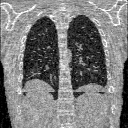
\includegraphics[width=\tempdima,height=\tempdima]{figures/experiments/xcat/fbp_coronal.png}
                                        };
                                        \spy [yellow] on (0.35,-0.3) in node [left,yellow] at (1.2, 1.0);
                                \end{scope}
                        \end{tikzpicture}
                \end{subfigure}
                \begin{subfigure}{0.19\linewidth}
                        \begin{tikzpicture}
                                \begin{scope}[spy using outlines={rounded rectangle, magnification=2, width=1.0cm, height=0.75cm, connect spies}]
                                        \node[inner sep=0pt] {
                                                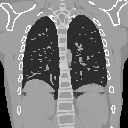
\includegraphics[width=\tempdima,height=\tempdima]{figures/experiments/xcat/gated_dps_coronal.png}
                                        };
                                        \spy [yellow] on (0.35,-0.3) in node [left,yellow] at (1.2, 1.0);
                                \end{scope}
                        \end{tikzpicture}
                \end{subfigure}
                \begin{subfigure}{0.19\linewidth}
                        \begin{tikzpicture}
                                \begin{scope}[spy using outlines={rounded rectangle, magnification=2, width=1.0cm, height=0.75cm, connect spies}]
                                        \node[inner sep=0pt] {
                                                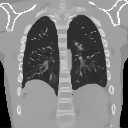
\includegraphics[width=\tempdima,height=\tempdima]{figures/experiments/xcat/blind_tv_coronal.png}
                                        };
                                        \spy [yellow] on (0.35,-0.3) in node [left,yellow] at (1.2, 1.0);
                                \end{scope}
                        \end{tikzpicture}
                \end{subfigure}
                \begin{subfigure}{0.19\linewidth}
                        \begin{tikzpicture}
                                \begin{scope}[spy using outlines={rounded rectangle, magnification=2, width=1.0cm, height=0.75cm, connect spies}]
                                        \node[inner sep=0pt] {
                                                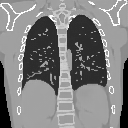
\includegraphics[width=\tempdima,height=\tempdima]{figures/experiments/xcat/blind_dps_coronal.png}
                                        };
                                        \spy [yellow] on (0.35,-0.3) in node [left,yellow] at (1.2, 1.0);
                                \end{scope}
                        \end{tikzpicture}
                \end{subfigure}
                \begin{subfigure}{0.19\linewidth}
                        \begin{tikzpicture}
                                \begin{scope}[spy using outlines={rounded rectangle, magnification=2, width=1.0cm, height=0.75cm, connect spies}]
                                        \node[inner sep=0pt] {
                                                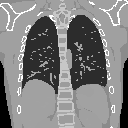
\includegraphics[width=\tempdima,height=\tempdima]{figures/experiments/xcat/gt_coronal.png}
                                        };
                                        \spy [yellow] on (0.35,-0.3) in node [left,yellow] at (1.2, 1.0);
                                \end{scope}
                        \end{tikzpicture}
                \end{subfigure}


                \begin{subfigure}{0.19\linewidth}
                        \begin{tikzpicture}
                                \begin{scope}[spy using outlines={rounded rectangle, magnification=2, width=1.0cm, height=0.75cm, connect spies}]
                                        \node[inner sep=0pt] {
                                                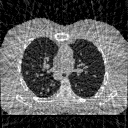
\includegraphics[width=\tempdima,height=\tempdima]{figures/experiments/xcat/fbp_axial.png}
                                        };
                                        \spy [yellow] on (0.05,-0.4) in node [left,yellow] at (1.2, 1.0);
                                \end{scope}
                        \end{tikzpicture}
                        \caption{\scriptsize Gated FBP}
                \end{subfigure}
                \begin{subfigure}{0.19\linewidth}
                        \begin{tikzpicture}
                                \begin{scope}[spy using outlines={rounded rectangle, magnification=2, width=1.0cm, height=0.75cm, connect spies}]
                                        \node[inner sep=0pt] {
                                                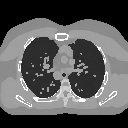
\includegraphics[width=\tempdima,height=\tempdima]{figures/experiments/xcat/gated_dps_axial.png}
                                        };
                                        \spy [yellow] on (0.05,-0.4) in node [left,yellow] at (1.2, 1.0);
                                \end{scope}
                        \end{tikzpicture}
                        \caption{\scriptsize Gated DPS}
                \end{subfigure}
                \begin{subfigure}{0.19\linewidth}
                        \begin{tikzpicture}
                                \begin{scope}[spy using outlines={rounded rectangle, magnification=2, width=1.0cm, height=0.75cm, connect spies}]
                                        \node[inner sep=0pt] {
                                                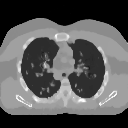
\includegraphics[width=\tempdima,height=\tempdima]{figures/experiments/xcat/blind_tv_axial.png}
                                        };
                                        \spy [yellow] on (0.05,-0.4) in node [left,yellow] at (1.2, 1.0);
                                \end{scope}
                        \end{tikzpicture}
                        \caption{\scriptsize JRM-TV}
                \end{subfigure}
                \begin{subfigure}{0.19\linewidth}
                        \begin{tikzpicture}
                                \begin{scope}[spy using outlines={rounded rectangle, magnification=2, width=1.0cm, height=0.75cm, connect spies}]
                                        \node[inner sep=0pt] {
                                                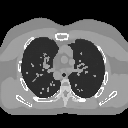
\includegraphics[width=\tempdima,height=\tempdima]{figures/experiments/xcat/blind_dps_axial.png}
                                        };
                                        \spy [yellow] on (0.05,-0.4) in node [left,yellow] at (1.2, 1.0);
                                \end{scope}
                        \end{tikzpicture}
                        \caption{\scriptsize JRM-ADM}
                \end{subfigure}
                \begin{subfigure}{0.19\linewidth}
                        \begin{tikzpicture}
                                \begin{scope}[spy using outlines={rounded rectangle, magnification=2, width=1.0cm, height=0.75cm, connect spies}]
                                        \node[inner sep=0pt] {
                                                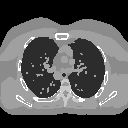
\includegraphics[width=\tempdima,height=\tempdima]{figures/experiments/xcat/gt_axial.png}
                                        };
                                        \spy [yellow] on (0.05,-0.4) in node [left,yellow] at (1.2, 1.0);
                                \end{scope}
                        \end{tikzpicture}
                        \caption{\scriptsize GT}
                \end{subfigure}

                \caption{
                        GT and end-inhale phase reconstructions on XCAT phantoms.
                }\label{fig:recon_xcat}

        \end{figure}

\end{frame}


\newlength{\reconimgsize}
\setlength{\reconimgsize}{0.17\linewidth}



\begin{frame}[fragile]
        \frametitle{Qualitative Evaluation of Reconstruction Methods}

        % %\newlength{\tempdima}
        % \setlength{\tempdima}{0.16\linewidth}



        % \only<1>{\begin{figure}
        %         \centering

        %         \begin{subfigure}{0.19\linewidth}
        %                 \begin{tikzpicture}
        %                         \begin{scope}[spy using outlines={rounded rectangle, magnification=2, width=1.0cm, height=0.75cm, connect spies}]
        %                                 \node[inner sep=0pt] {
        %                                         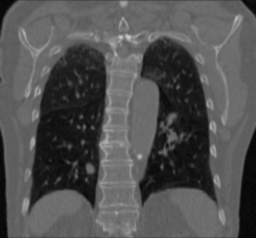
\includegraphics[width=\tempdima,height=\tempdima]{figures/experiments/recon_lung/gt_cor_0.png}
        %                                 };
        %                                 \spy [yellow] on (0.35,-0.3) in node [left,yellow] at (1.2, 1.0);
        %                         \end{scope}
        %                 \end{tikzpicture}
        %         \end{subfigure}
        %         \begin{subfigure}{0.19\linewidth}
        %                 \begin{tikzpicture}
        %                         \begin{scope}[spy using outlines={rounded rectangle, magnification=2, width=1.0cm, height=0.75cm, connect spies}]
        %                                 \node[inner sep=0pt] {
        %                                         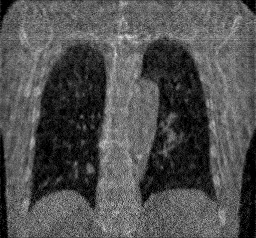
\includegraphics[width=\tempdima,height=\tempdima]{figures/experiments/recon_lung/fbp_cor_0.png}
        %                                 };
        %                                 \spy [yellow] on (0.35,-0.3) in node [left,yellow] at (1.2, 1.0);
        %                         \end{scope}
        %                 \end{tikzpicture}
        %         \end{subfigure}
        %         \begin{subfigure}{0.19\linewidth}
        %                 \begin{tikzpicture}
        %                         \begin{scope}[spy using outlines={rounded rectangle, magnification=2, width=1.0cm, height=0.75cm, connect spies}]
        %                                 \node[inner sep=0pt] {
        %                                         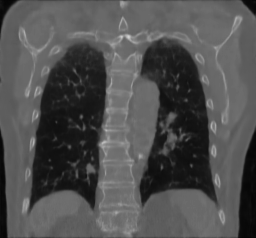
\includegraphics[width=\tempdima,height=\tempdima]{figures/experiments/recon_lung/gated_dps_cor_0.png}
        %                                 };
        %                                 \spy [yellow] on (0.35,-0.3) in node [left,yellow] at (1.2, 1.0);
        %                         \end{scope}
        %                 \end{tikzpicture}
        %         \end{subfigure}
        %         \begin{subfigure}{0.19\linewidth}
        %                 \begin{tikzpicture}
        %                         \begin{scope}[spy using outlines={rounded rectangle, magnification=2, width=1.0cm, height=0.75cm, connect spies}]
        %                                 \node[inner sep=0pt] {
        %                                         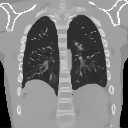
\includegraphics[width=\tempdima,height=\tempdima]{figures/experiments/xcat/blind_tv_coronal.png}
        %                                 };
        %                                 \spy [yellow] on (0.35,-0.3) in node [left,yellow] at (1.2, 1.0);
        %                         \end{scope}
        %                 \end{tikzpicture}
        %         \end{subfigure}
        %         \begin{subfigure}{0.19\linewidth}
        %                 \begin{tikzpicture}
        %                         \begin{scope}[spy using outlines={rounded rectangle, magnification=2, width=1.0cm, height=0.75cm, connect spies}]
        %                                 \node[inner sep=0pt] {
        %                                         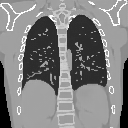
\includegraphics[width=\tempdima,height=\tempdima]{figures/experiments/xcat/blind_dps_coronal.png}
        %                                 };
        %                                 \spy [yellow] on (0.35,-0.3) in node [left,yellow] at (1.2, 1.0);
        %                         \end{scope}
        %                 \end{tikzpicture}
        %         \end{subfigure}


        %         \begin{subfigure}{0.19\linewidth}
        %                 \begin{tikzpicture}
        %                         \begin{scope}[spy using outlines={rounded rectangle, magnification=2, width=1.0cm, height=0.75cm, connect spies}]
        %                                 \node[inner sep=0pt] {
        %                                         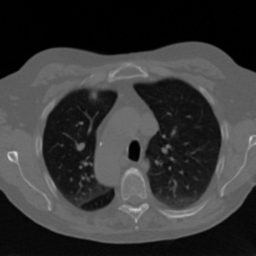
\includegraphics[width=\tempdima,height=\tempdima]{figures/experiments/recon_lung/gt_axe_0.png}
        %                                 };
        %                                 \spy [yellow] on (0.05,-0.4) in node [left,yellow] at (1.2, 1.0);
        %                         \end{scope}
        %                 \end{tikzpicture}
        %                 \caption{GT}
        %         \end{subfigure}
        %         \begin{subfigure}{0.19\linewidth}
        %                 \begin{tikzpicture}
        %                         \begin{scope}[spy using outlines={rounded rectangle, magnification=2, width=1.0cm, height=0.75cm, connect spies}]
        %                                 \node[inner sep=0pt] {
        %                                         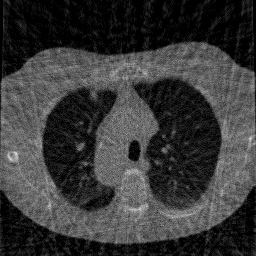
\includegraphics[width=\tempdima,height=\tempdima]{figures/experiments/recon_lung/fbp_axe_0.png}
        %                                 };
        %                                 \spy [yellow] on (0.05,-0.4) in node [left,yellow] at (1.2, 1.0);
        %                         \end{scope}
        %                 \end{tikzpicture}
        %                 \caption{Gated FBP}
        %         \end{subfigure}
        %         \begin{subfigure}{0.19\linewidth}
        %                 \begin{tikzpicture}
        %                         \begin{scope}[spy using outlines={rounded rectangle, magnification=2, width=1.0cm, height=0.75cm, connect spies}]
        %                                 \node[inner sep=0pt] {
        %                                         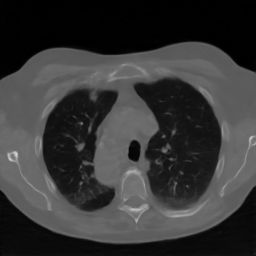
\includegraphics[width=\tempdima,height=\tempdima]{figures/experiments/recon_lung/gated_dps_axe_0.png}
        %                                 };
        %                                 \spy [yellow] on (0.05,-0.4) in node [left,yellow] at (1.2, 1.0);
        %                         \end{scope}
        %                 \end{tikzpicture}
        %                 \caption{Gated DPS}
        %         \end{subfigure}
        %         \begin{subfigure}{0.19\linewidth}
        %                 \begin{tikzpicture}
        %                         \begin{scope}[spy using outlines={rounded rectangle, magnification=2, width=1.0cm, height=0.75cm, connect spies}]
        %                                 \node[inner sep=0pt] {
        %                                         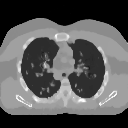
\includegraphics[width=\tempdima,height=\tempdima]{figures/experiments/xcat/blind_tv_axial.png}
        %                                 };
        %                                 \spy [yellow] on (0.05,-0.4) in node [left,yellow] at (1.2, 1.0);
        %                         \end{scope}
        %                 \end{tikzpicture}
        %                 \caption{JRM-TV}
        %         \end{subfigure}
        %         \begin{subfigure}{0.19\linewidth}
        %                 \begin{tikzpicture}
        %                         \begin{scope}[spy using outlines={rounded rectangle, magnification=2, width=1.0cm, height=0.75cm, connect spies}]
        %                                 \node[inner sep=0pt] {
        %                                         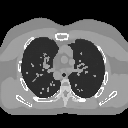
\includegraphics[width=\tempdima,height=\tempdima]{figures/experiments/xcat/blind_dps_axial.png}
        %                                 };
        %                                 \spy [yellow] on (0.05,-0.4) in node [left,yellow] at (1.2, 1.0);
        %                         \end{scope}
        %                 \end{tikzpicture}
        %                 \caption{JRM-ADM}
        %         \end{subfigure}

        %         \caption{
        %                 GT and end-inhale phase reconstructions on XCAT phantom.
        %         }
        % \end{figure}}


        %         \only<2>{\begin{figure}
        %         \centering

        %         \begin{subfigure}{0.19\linewidth}
        %                 \begin{tikzpicture}
        %                         \begin{scope}[spy using outlines={rounded rectangle, magnification=2, width=1.0cm, height=0.75cm, connect spies}]
        %                                 \node[inner sep=0pt] {
        %                                         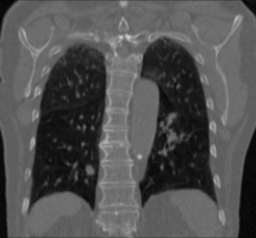
\includegraphics[width=\tempdima,height=\tempdima]{figures/experiments/recon_lung/gt_cor_1.png}
        %                                 };
        %                                 \spy [yellow] on (0.35,-0.3) in node [left,yellow] at (1.2, 1.0);
        %                         \end{scope}
        %                 \end{tikzpicture}
        %         \end{subfigure}
        %         \begin{subfigure}{0.19\linewidth}
        %                 \begin{tikzpicture}
        %                         \begin{scope}[spy using outlines={rounded rectangle, magnification=2, width=1.0cm, height=0.75cm, connect spies}]
        %                                 \node[inner sep=0pt] {
        %                                         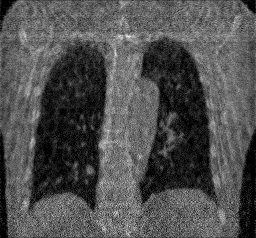
\includegraphics[width=\tempdima,height=\tempdima]{figures/experiments/recon_lung/fbp_cor_1.png}
        %                                 };
        %                                 \spy [yellow] on (0.35,-0.3) in node [left,yellow] at (1.2, 1.0);
        %                         \end{scope}
        %                 \end{tikzpicture}
        %         \end{subfigure}
        %         \begin{subfigure}{0.19\linewidth}
        %                 \begin{tikzpicture}
        %                         \begin{scope}[spy using outlines={rounded rectangle, magnification=2, width=1.0cm, height=0.75cm, connect spies}]
        %                                 \node[inner sep=0pt] {
        %                                         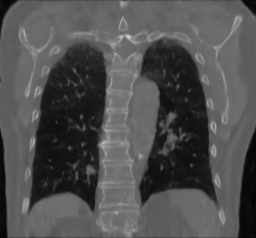
\includegraphics[width=\tempdima,height=\tempdima]{figures/experiments/recon_lung/gated_dps_cor_1.png}
        %                                 };
        %                                 \spy [yellow] on (0.35,-0.3) in node [left,yellow] at (1.2, 1.0);
        %                         \end{scope}
        %                 \end{tikzpicture}
        %         \end{subfigure}
        %         \begin{subfigure}{0.19\linewidth}
        %                 \begin{tikzpicture}
        %                         \begin{scope}[spy using outlines={rounded rectangle, magnification=2, width=1.0cm, height=0.75cm, connect spies}]
        %                                 \node[inner sep=0pt] {
        %                                         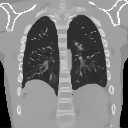
\includegraphics[width=\tempdima,height=\tempdima]{figures/experiments/xcat/blind_tv_coronal.png}
        %                                 };
        %                                 \spy [yellow] on (0.35,-0.3) in node [left,yellow] at (1.2, 1.0);
        %                         \end{scope}
        %                 \end{tikzpicture}
        %         \end{subfigure}
        %         \begin{subfigure}{0.19\linewidth}
        %                 \begin{tikzpicture}
        %                         \begin{scope}[spy using outlines={rounded rectangle, magnification=2, width=1.0cm, height=0.75cm, connect spies}]
        %                                 \node[inner sep=0pt] {
        %                                         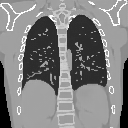
\includegraphics[width=\tempdima,height=\tempdima]{figures/experiments/xcat/blind_dps_coronal.png}
        %                                 };
        %                                 \spy [yellow] on (0.35,-0.3) in node [left,yellow] at (1.2, 1.0);
        %                         \end{scope}
        %                 \end{tikzpicture}
        %         \end{subfigure}


        %         \begin{subfigure}{0.19\linewidth}
        %                 \begin{tikzpicture}
        %                         \begin{scope}[spy using outlines={rounded rectangle, magnification=2, width=1.0cm, height=0.75cm, connect spies}]
        %                                 \node[inner sep=0pt] {
        %                                         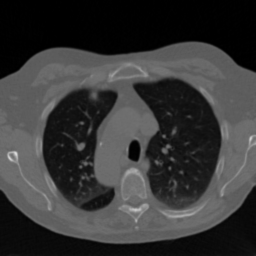
\includegraphics[width=\tempdima,height=\tempdima]{figures/experiments/recon_lung/gt_axe_1.png}
        %                                 };
        %                                 \spy [yellow] on (0.05,-0.4) in node [left,yellow] at (1.2, 1.0);
        %                         \end{scope}
        %                 \end{tikzpicture}
        %                 \caption{GT}
        %         \end{subfigure}
        %         \begin{subfigure}{0.19\linewidth}
        %                 \begin{tikzpicture}
        %                         \begin{scope}[spy using outlines={rounded rectangle, magnification=2, width=1.0cm, height=0.75cm, connect spies}]
        %                                 \node[inner sep=0pt] {
        %                                         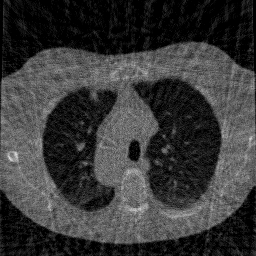
\includegraphics[width=\tempdima,height=\tempdima]{figures/experiments/recon_lung/fbp_axe_1.png}
        %                                 };
        %                                 \spy [yellow] on (0.05,-0.4) in node [left,yellow] at (1.2, 1.0);
        %                         \end{scope}
        %                 \end{tikzpicture}
        %                 \caption{Gated FBP}
        %         \end{subfigure}
        %         \begin{subfigure}{0.19\linewidth}
        %                 \begin{tikzpicture}
        %                         \begin{scope}[spy using outlines={rounded rectangle, magnification=2, width=1.0cm, height=0.75cm, connect spies}]
        %                                 \node[inner sep=0pt] {
        %                                         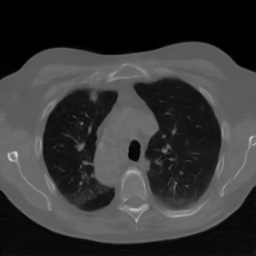
\includegraphics[width=\tempdima,height=\tempdima]{figures/experiments/recon_lung/gated_dps_axe_1.png}
        %                                 };
        %                                 \spy [yellow] on (0.05,-0.4) in node [left,yellow] at (1.2, 1.0);
        %                         \end{scope}
        %                 \end{tikzpicture}
        %                 \caption{Gated DPS}
        %         \end{subfigure}
        %         \begin{subfigure}{0.19\linewidth}
        %                 \begin{tikzpicture}
        %                         \begin{scope}[spy using outlines={rounded rectangle, magnification=2, width=1.0cm, height=0.75cm, connect spies}]
        %                                 \node[inner sep=0pt] {
        %                                         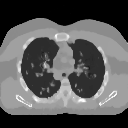
\includegraphics[width=\tempdima,height=\tempdima]{figures/experiments/xcat/blind_tv_axial.png}
        %                                 };
        %                                 \spy [yellow] on (0.05,-0.4) in node [left,yellow] at (1.2, 1.0);
        %                         \end{scope}
        %                 \end{tikzpicture}
        %                 \caption{JRM-TV}
        %         \end{subfigure}
        %         \begin{subfigure}{0.19\linewidth}
        %                 \begin{tikzpicture}
        %                         \begin{scope}[spy using outlines={rounded rectangle, magnification=2, width=1.0cm, height=0.75cm, connect spies}]
        %                                 \node[inner sep=0pt] {
        %                                         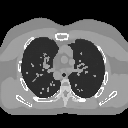
\includegraphics[width=\tempdima,height=\tempdima]{figures/experiments/xcat/blind_dps_axial.png}
        %                                 };
        %                                 \spy [yellow] on (0.05,-0.4) in node [left,yellow] at (1.2, 1.0);
        %                         \end{scope}
        %                 \end{tikzpicture}
        %                 \caption{JRM-ADM}
        %         \end{subfigure}

        %         \caption{
        %                 GT and end-inhale phase reconstructions on XCAT phantom.
        %         }
        % \end{figure}}


% use a fresh length name and make it slightly smaller

\newcommand{\ReconSubFig}[4][]{%
  \begin{subfigure}{\reconimgsize}
    \begin{tikzpicture}
      \begin{scope}[spy using outlines={
                        rounded rectangle,
                        magnification=2,
                        width=1.0cm,
                        height=0.75cm,
                        connect spies}]
        \node[inner sep=0pt]{%
          \includegraphics[width=\reconimgsize,height=\reconimgsize]{#2}%
        };
        \spy[yellow] on #3 in node[left,yellow] at #4;
      \end{scope}
    \end{tikzpicture}
    \ifx&#1&\else\caption{\scriptsize #1}\fi
  \end{subfigure}%
}


\only<1>{%
  \begin{figure}
    \centering
    % Coronal views (GT last)
    \makebox[\linewidth][c]{%
      \ReconSubFig{figures/experiments/recon_lung/fbp_cor_0.png}{(0.35,-0.6)}{(1.2,1.0)}\hfill
      \ReconSubFig{figures/experiments/recon_lung/gated_dps_cor_0.png}{(0.35,-0.6)}{(1.2,1.0)}\hfill
      \ReconSubFig{figures/experiments/recon_lung/jrm_tv_cor_0.png}{(0.35,-0.6)}{(1.2,1.0)}\hfill
      \ReconSubFig{figures/experiments/recon_lung/jrm_adm_cor_0.png}{(0.35,-0.6)}{(1.2,1.0)}\hfill
      \ReconSubFig{figures/experiments/recon_lung/gt_cor_0.png}{(0.35,-0.6)}{(1.2,1.0)}%
    }
    % Axial views (GT last)
    \makebox[\linewidth][c]{%
      \ReconSubFig[Gated FBP]{figures/experiments/recon_lung/fbp_axe_0.png}{(0.05,-0.4)}{(1.2,1.0)}\hfill
      \ReconSubFig[Gated DPS]{figures/experiments/recon_lung/gated_dps_axe_0.png}{(0.05,-0.4)}{(1.2,1.0)}\hfill
      \ReconSubFig[JRM-TV]{figures/experiments/recon_lung/jrm_tv_axe_0.png}{(0.05,-0.4)}{(1.2,1.0)}\hfill
      \ReconSubFig[JRM-ADM]{figures/experiments/recon_lung/jrm_adm_axe_0.png}{(0.05,-0.4)}{(1.2,1.0)}\hfill
      \ReconSubFig[GT]{figures/experiments/recon_lung/gt_axe_0.png}{(0.05,-0.4)}{(1.2,1.0)}%
    }
    \caption{GT and reconstructions on pseudo-real data.}
  \end{figure}%
}

\only<2>{%
  \begin{figure}
    \centering
    \makebox[\linewidth][c]{%
      \ReconSubFig{figures/experiments/recon_lung/fbp_cor_1.png}{(0.35,-0.6)}{(1.2,1.0)}\hfill
      \ReconSubFig{figures/experiments/recon_lung/gated_dps_cor_1.png}{(0.35,-0.6)}{(1.2,1.0)}\hfill
      \ReconSubFig{figures/experiments/recon_lung/jrm_tv_cor_1.png}{(0.35,-0.6)}{(1.2,1.0)}\hfill
      \ReconSubFig{figures/experiments/recon_lung/jrm_adm_cor_1.png}{(0.35,-0.6)}{(1.2,1.0)}\hfill
      \ReconSubFig{figures/experiments/recon_lung/gt_cor_1.png}{(0.35,-0.6)}{(1.2,1.0)}%
    }
    \makebox[\linewidth][c]{%
      \ReconSubFig[Gated FBP]{figures/experiments/recon_lung/fbp_axe_1.png}{(0.05,-0.4)}{(1.2,1.0)}\hfill
      \ReconSubFig[Gated DPS]{figures/experiments/recon_lung/gated_dps_axe_1.png}{(0.05,-0.4)}{(1.2,1.0)}\hfill
      \ReconSubFig[JRM-TV]{figures/experiments/recon_lung/jrm_tv_axe_1.png}{(0.05,-0.4)}{(1.2,1.0)}\hfill
      \ReconSubFig[JRM-ADM]{figures/experiments/recon_lung/jrm_adm_axe_1.png}{(0.05,-0.4)}{(1.2,1.0)}\hfill
      \ReconSubFig[GT]{figures/experiments/recon_lung/gt_axe_1.png}{(0.05,-0.4)}{(1.2,1.0)}%
    }
    \caption{GT and reconstructions on pseudo-real data.}
  \end{figure}%
}

\only<3>{%
  \begin{figure}
    \centering
    \makebox[\linewidth][c]{%
      \ReconSubFig{figures/experiments/recon_lung/fbp_cor_2.png}{(0.35,-0.6)}{(1.2,1.0)}\hfill
      \ReconSubFig{figures/experiments/recon_lung/gated_dps_cor_2.png}{(0.35,-0.6)}{(1.2,1.0)}\hfill
      \ReconSubFig{figures/experiments/recon_lung/jrm_tv_cor_2.png}{(0.35,-0.6)}{(1.2,1.0)}\hfill
      \ReconSubFig{figures/experiments/recon_lung/jrm_adm_cor_2.png}{(0.35,-0.6)}{(1.2,1.0)}\hfill
      \ReconSubFig{figures/experiments/recon_lung/gt_cor_2.png}{(0.35,-0.6)}{(1.2,1.0)}%
    }
    \makebox[\linewidth][c]{%
      \ReconSubFig[Gated FBP]{figures/experiments/recon_lung/fbp_axe_2.png}{(0.05,-0.4)}{(1.2,1.0)}\hfill
      \ReconSubFig[Gated DPS]{figures/experiments/recon_lung/gated_dps_axe_2.png}{(0.05,-0.4)}{(1.2,1.0)}\hfill
      \ReconSubFig[JRM-TV]{figures/experiments/recon_lung/jrm_tv_axe_2.png}{(0.05,-0.4)}{(1.2,1.0)}\hfill
      \ReconSubFig[JRM-ADM]{figures/experiments/recon_lung/jrm_adm_axe_2.png}{(0.05,-0.4)}{(1.2,1.0)}\hfill
      \ReconSubFig[GT]{figures/experiments/recon_lung/gt_axe_2.png}{(0.05,-0.4)}{(1.2,1.0)}%
    }
    \caption{GT and reconstructions on pseudo-real data.}
  \end{figure}%
}

\only<4>{%
  \begin{figure}
    \centering
    \makebox[\linewidth][c]{%
      \ReconSubFig{figures/experiments/recon_lung/fbp_cor_3.png}{(0.35,-0.6)}{(1.2,1.0)}\hfill
      \ReconSubFig{figures/experiments/recon_lung/gated_dps_cor_3.png}{(0.35,-0.6)}{(1.2,1.0)}\hfill
      \ReconSubFig{figures/experiments/recon_lung/jrm_tv_cor_3.png}{(0.35,-0.6)}{(1.2,1.0)}\hfill
      \ReconSubFig{figures/experiments/recon_lung/jrm_adm_cor_3.png}{(0.35,-0.6)}{(1.2,1.0)}\hfill
      \ReconSubFig{figures/experiments/recon_lung/gt_cor_3.png}{(0.35,-0.6)}{(1.2,1.0)}%
    }
    \makebox[\linewidth][c]{%
      \ReconSubFig[Gated FBP]{figures/experiments/recon_lung/fbp_axe_3.png}{(0.05,-0.4)}{(1.2,1.0)}\hfill
      \ReconSubFig[Gated DPS]{figures/experiments/recon_lung/gated_dps_axe_3.png}{(0.05,-0.4)}{(1.2,1.0)}\hfill
      \ReconSubFig[JRM-TV]{figures/experiments/recon_lung/jrm_tv_axe_3.png}{(0.05,-0.4)}{(1.2,1.0)}\hfill
      \ReconSubFig[JRM-ADM]{figures/experiments/recon_lung/jrm_adm_axe_3.png}{(0.05,-0.4)}{(1.2,1.0)}\hfill
      \ReconSubFig[GT]{figures/experiments/recon_lung/gt_axe_3.png}{(0.05,-0.4)}{(1.2,1.0)}%
    }
    \caption{GT and reconstructions on pseudo-real data.}
  \end{figure}%
}

\only<5>{%
  \begin{figure}
    \centering
    \makebox[\linewidth][c]{%
      \ReconSubFig{figures/experiments/recon_lung/fbp_cor_4.png}{(0.35,-0.6)}{(1.2,1.0)}\hfill
      \ReconSubFig{figures/experiments/recon_lung/gated_dps_cor_4.png}{(0.35,-0.6)}{(1.2,1.0)}\hfill
      \ReconSubFig{figures/experiments/recon_lung/jrm_tv_cor_4.png}{(0.35,-0.6)}{(1.2,1.0)}\hfill
      \ReconSubFig{figures/experiments/recon_lung/jrm_adm_cor_4.png}{(0.35,-0.6)}{(1.2,1.0)}\hfill
      \ReconSubFig{figures/experiments/recon_lung/gt_cor_4.png}{(0.35,-0.6)}{(1.2,1.0)}%
    }
    \makebox[\linewidth][c]{%
      \ReconSubFig[Gated FBP]{figures/experiments/recon_lung/fbp_axe_4.png}{(0.05,-0.4)}{(1.2,1.0)}\hfill
      \ReconSubFig[Gated DPS]{figures/experiments/recon_lung/gated_dps_axe_4.png}{(0.05,-0.4)}{(1.2,1.0)}\hfill
      \ReconSubFig[JRM-TV]{figures/experiments/recon_lung/jrm_tv_axe_4.png}{(0.05,-0.4)}{(1.2,1.0)}\hfill
      \ReconSubFig[JRM-ADM]{figures/experiments/recon_lung/jrm_adm_axe_4.png}{(0.05,-0.4)}{(1.2,1.0)}\hfill
      \ReconSubFig[GT]{figures/experiments/recon_lung/gt_axe_4.png}{(0.05,-0.4)}{(1.2,1.0)}%
    }
    \caption{GT and reconstructions on pseudo-real data.}
  \end{figure}%
}

\only<6>{%
  \begin{figure}
    \centering
    \makebox[\linewidth][c]{%
      \ReconSubFig{figures/experiments/recon_lung/fbp_cor_5.png}{(0.35,-0.6)}{(1.2,1.0)}\hfill
      \ReconSubFig{figures/experiments/recon_lung/gated_dps_cor_5.png}{(0.35,-0.6)}{(1.2,1.0)}\hfill
      \ReconSubFig{figures/experiments/recon_lung/jrm_tv_cor_5.png}{(0.35,-0.6)}{(1.2,1.0)}\hfill
      \ReconSubFig{figures/experiments/recon_lung/jrm_adm_cor_5.png}{(0.35,-0.6)}{(1.2,1.0)}\hfill
      \ReconSubFig{figures/experiments/recon_lung/gt_cor_5.png}{(0.35,-0.6)}{(1.2,1.0)}%
    }
    \makebox[\linewidth][c]{%
      \ReconSubFig[Gated FBP]{figures/experiments/recon_lung/fbp_axe_5.png}{(0.05,-0.4)}{(1.2,1.0)}\hfill
      \ReconSubFig[Gated DPS]{figures/experiments/recon_lung/gated_dps_axe_5.png}{(0.05,-0.4)}{(1.2,1.0)}\hfill
      \ReconSubFig[JRM-TV]{figures/experiments/recon_lung/jrm_tv_axe_5.png}{(0.05,-0.4)}{(1.2,1.0)}\hfill
      \ReconSubFig[JRM-ADM]{figures/experiments/recon_lung/jrm_adm_axe_5.png}{(0.05,-0.4)}{(1.2,1.0)}\hfill
      \ReconSubFig[GT]{figures/experiments/recon_lung/gt_axe_5.png}{(0.05,-0.4)}{(1.2,1.0)}%
    }
    \caption{GT and reconstructions on pseudo-real data.}
  \end{figure}%
}

\only<7>{%
  \begin{figure}
    \centering
    \makebox[\linewidth][c]{%
      \ReconSubFig{figures/experiments/recon_lung/fbp_cor_6.png}{(0.35,-0.6)}{(1.2,1.0)}\hfill
      \ReconSubFig{figures/experiments/recon_lung/gated_dps_cor_6.png}{(0.35,-0.6)}{(1.2,1.0)}\hfill
      \ReconSubFig{figures/experiments/recon_lung/jrm_tv_cor_6.png}{(0.35,-0.6)}{(1.2,1.0)}\hfill
      \ReconSubFig{figures/experiments/recon_lung/jrm_adm_cor_6.png}{(0.35,-0.6)}{(1.2,1.0)}\hfill
      \ReconSubFig{figures/experiments/recon_lung/gt_cor_6.png}{(0.35,-0.6)}{(1.2,1.0)}%
    }
    \makebox[\linewidth][c]{%
      \ReconSubFig[Gated FBP]{figures/experiments/recon_lung/fbp_axe_6.png}{(0.05,-0.4)}{(1.2,1.0)}\hfill
      \ReconSubFig[Gated DPS]{figures/experiments/recon_lung/gated_dps_axe_6.png}{(0.05,-0.4)}{(1.2,1.0)}\hfill
      \ReconSubFig[JRM-TV]{figures/experiments/recon_lung/jrm_tv_axe_6.png}{(0.05,-0.4)}{(1.2,1.0)}\hfill
      \ReconSubFig[JRM-ADM]{figures/experiments/recon_lung/jrm_adm_axe_6.png}{(0.05,-0.4)}{(1.2,1.0)}\hfill
      \ReconSubFig[GT]{figures/experiments/recon_lung/gt_axe_6.png}{(0.05,-0.4)}{(1.2,1.0)}%
    }
    \caption{GT and reconstructions on pseudo-real data.}
  \end{figure}%
}

\only<8>{%
  \begin{figure}
    \centering
    \makebox[\linewidth][c]{%
      \ReconSubFig{figures/experiments/recon_lung/fbp_cor_7.png}{(0.35,-0.6)}{(1.2,1.0)}\hfill
      \ReconSubFig{figures/experiments/recon_lung/gated_dps_cor_7.png}{(0.35,-0.6)}{(1.2,1.0)}\hfill
      \ReconSubFig{figures/experiments/recon_lung/jrm_tv_cor_7.png}{(0.35,-0.6)}{(1.2,1.0)}\hfill
      \ReconSubFig{figures/experiments/recon_lung/jrm_adm_cor_7.png}{(0.35,-0.6)}{(1.2,1.0)}\hfill
      \ReconSubFig{figures/experiments/recon_lung/gt_cor_7.png}{(0.35,-0.6)}{(1.2,1.0)}%
    }
    \makebox[\linewidth][c]{%
      \ReconSubFig[Gated FBP]{figures/experiments/recon_lung/fbp_axe_7.png}{(0.05,-0.4)}{(1.2,1.0)}\hfill
      \ReconSubFig[Gated DPS]{figures/experiments/recon_lung/gated_dps_axe_7.png}{(0.05,-0.4)}{(1.2,1.0)}\hfill
      \ReconSubFig[JRM-TV]{figures/experiments/recon_lung/jrm_tv_axe_7.png}{(0.05,-0.4)}{(1.2,1.0)}\hfill
      \ReconSubFig[JRM-ADM]{figures/experiments/recon_lung/jrm_adm_axe_7.png}{(0.05,-0.4)}{(1.2,1.0)}\hfill
      \ReconSubFig[GT]{figures/experiments/recon_lung/gt_axe_7.png}{(0.05,-0.4)}{(1.2,1.0)}%
    }
    \caption{GT and reconstructions on pseudo-real data.}
  \end{figure}%
}

\only<9>{%
  \begin{figure}
    \centering
    \makebox[\linewidth][c]{%
      \ReconSubFig{figures/experiments/recon_lung/fbp_cor_8.png}{(0.35,-0.6)}{(1.2,1.0)}\hfill
      \ReconSubFig{figures/experiments/recon_lung/gated_dps_cor_8.png}{(0.35,-0.6)}{(1.2,1.0)}\hfill
      \ReconSubFig{figures/experiments/recon_lung/jrm_tv_cor_8.png}{(0.35,-0.6)}{(1.2,1.0)}\hfill
      \ReconSubFig{figures/experiments/recon_lung/jrm_adm_cor_8.png}{(0.35,-0.6)}{(1.2,1.0)}\hfill
      \ReconSubFig{figures/experiments/recon_lung/gt_cor_8.png}{(0.35,-0.6)}{(1.2,1.0)}%
    }
    \makebox[\linewidth][c]{%
      \ReconSubFig[Gated FBP]{figures/experiments/recon_lung/fbp_axe_8.png}{(0.05,-0.4)}{(1.2,1.0)}\hfill
      \ReconSubFig[Gated DPS]{figures/experiments/recon_lung/gated_dps_axe_8.png}{(0.05,-0.4)}{(1.2,1.0)}\hfill
      \ReconSubFig[JRM-TV]{figures/experiments/recon_lung/jrm_tv_axe_8.png}{(0.05,-0.4)}{(1.2,1.0)}\hfill
      \ReconSubFig[JRM-ADM]{figures/experiments/recon_lung/jrm_adm_axe_8.png}{(0.05,-0.4)}{(1.2,1.0)}\hfill
      \ReconSubFig[GT]{figures/experiments/recon_lung/gt_axe_8.png}{(0.05,-0.4)}{(1.2,1.0)}%
    }
    \caption{GT and reconstructions on pseudo-real data.}
  \end{figure}%
}

\only<10>{%
  \begin{figure}
    \centering
    \makebox[\linewidth][c]{%
      \ReconSubFig{figures/experiments/recon_lung/fbp_cor_9.png}{(0.35,-0.6)}{(1.2,1.0)}\hfill
      \ReconSubFig{figures/experiments/recon_lung/gated_dps_cor_9.png}{(0.35,-0.6)}{(1.2,1.0)}\hfill
      \ReconSubFig{figures/experiments/recon_lung/jrm_tv_cor_9.png}{(0.35,-0.6)}{(1.2,1.0)}\hfill
      \ReconSubFig{figures/experiments/recon_lung/jrm_adm_cor_9.png}{(0.35,-0.6)}{(1.2,1.0)}\hfill
      \ReconSubFig{figures/experiments/recon_lung/gt_cor_9.png}{(0.35,-0.6)}{(1.2,1.0)}%
    }
    \makebox[\linewidth][c]{%
      \ReconSubFig[Gated FBP]{figures/experiments/recon_lung/fbp_axe_9.png}{(0.05,-0.4)}{(1.2,1.0)}\hfill
      \ReconSubFig[Gated DPS]{figures/experiments/recon_lung/gated_dps_axe_9.png}{(0.05,-0.4)}{(1.2,1.0)}\hfill
      \ReconSubFig[JRM-TV]{figures/experiments/recon_lung/jrm_tv_axe_9.png}{(0.05,-0.4)}{(1.2,1.0)}\hfill
      \ReconSubFig[JRM-ADM]{figures/experiments/recon_lung/jrm_adm_axe_9.png}{(0.05,-0.4)}{(1.2,1.0)}\hfill
      \ReconSubFig[GT]{figures/experiments/recon_lung/gt_axe_9.png}{(0.05,-0.4)}{(1.2,1.0)}%
    }
    \caption{GT and reconstructions on pseudo-real data.}
  \end{figure}%
}


%   \only<1>{%
%     \begin{figure}
%       \centering
%       \makebox[\linewidth][c]{%
%         \ReconSubFig{figures/experiments/recon_lung/gt_cor_0.png}{(0.35,-0.6)}{(1.2,1.0)}\hfill
%         \ReconSubFig{figures/experiments/recon_lung/fbp_cor_0.png}{(0.35,-0.6)}{(1.2,1.0)}\hfill
%         \ReconSubFig{figures/experiments/recon_lung/gated_dps_cor_0.png}{(0.35,-0.6)}{(1.2,1.0)}\hfill
%         \ReconSubFig{figures/experiments/recon_lung/jrm_tv_cor_0.png}{(0.35,-0.6)}{(1.2,1.0)}\hfill
%         \ReconSubFig{figures/experiments/recon_lung/jrm_adm_cor_0.png}{(0.35,-0.6)}{(1.2,1.0)}%
%       }

%       \makebox[\linewidth][c]{%
%         \ReconSubFig[GT]{figures/experiments/recon_lung/gt_axe_0.png}{(0.05,-0.4)}{(1.2,1.0)}\hfill
%         \ReconSubFig[Gated FBP]{figures/experiments/recon_lung/fbp_axe_0.png}{(0.05,-0.4)}{(1.2,1.0)}\hfill
%         \ReconSubFig[Gated DPS]{figures/experiments/recon_lung/gated_dps_axe_0.png}{(0.05,-0.4)}{(1.2,1.0)}\hfill
%         \ReconSubFig[JRM-TV]{figures/experiments/recon_lung/jrm_tv_axe_0.png}{(0.05,-0.4)}{(1.2,1.0)}\hfill
%         \ReconSubFig[JRM-ADM]{figures/experiments/recon_lung/jrm_adm_axe_0.png}{(0.05,-0.4)}{(1.2,1.0)}%
%       }
%       \caption{GT and reconstructions on pseudo-real data.}
%     \end{figure}%
%   }

%   \only<2>{%
%     \begin{figure}
%       \centering
%       \makebox[\linewidth][c]{%
%         \ReconSubFig{figures/experiments/recon_lung/gt_cor_1.png}{(0.35,-0.6)}{(1.2,1.0)}\hfill
%         \ReconSubFig{figures/experiments/recon_lung/fbp_cor_1.png}{(0.35,-0.6)}{(1.2,1.0)}\hfill
%         \ReconSubFig{figures/experiments/recon_lung/gated_dps_cor_1.png}{(0.35,-0.6)}{(1.2,1.0)}\hfill
%         \ReconSubFig{figures/experiments/recon_lung/jrm_tv_cor_1.png}{(0.35,-0.6)}{(1.2,1.0)}\hfill
%         \ReconSubFig{figures/experiments/recon_lung/jrm_adm_cor_1.png}{(0.35,-0.6)}{(1.2,1.0)}%
%       }

%       \makebox[\linewidth][c]{%
%         \ReconSubFig[GT]{figures/experiments/recon_lung/gt_axe_1.png}{(0.05,-0.4)}{(1.2,1.0)}\hfill
%         \ReconSubFig[Gated FBP]{figures/experiments/recon_lung/fbp_axe_1.png}{(0.05,-0.4)}{(1.2,1.0)}\hfill
%         \ReconSubFig[Gated DPS]{figures/experiments/recon_lung/gated_dps_axe_1.png}{(0.05,-0.4)}{(1.2,1.0)}\hfill
%         \ReconSubFig[JRM-TV]{figures/experiments/recon_lung/jrm_tv_axe_1.png}{(0.05,-0.4)}{(1.2,1.0)}\hfill
%         \ReconSubFig[JRM-ADM]{figures/experiments/recon_lung/jrm_adm_axe_1.png}{(0.05,-0.4)}{(1.2,1.0)}%
%       }
%       \caption{GT and reconstructions on pseudo-real data.}
%     \end{figure}%
%   }

%     \only<3>{%
%     \begin{figure}
%       \centering
%       \makebox[\linewidth][c]{%
%         \ReconSubFig{figures/experiments/recon_lung/gt_cor_2.png}{(0.35,-0.6)}{(1.2,1.0)}\hfill
%         \ReconSubFig{figures/experiments/recon_lung/fbp_cor_2.png}{(0.35,-0.6)}{(1.2,1.0)}\hfill
%         \ReconSubFig{figures/experiments/recon_lung/gated_dps_cor_2.png}{(0.35,-0.6)}{(1.2,1.0)}\hfill
%         \ReconSubFig{figures/experiments/recon_lung/jrm_tv_cor_2.png}{(0.35,-0.6)}{(1.2,1.0)}\hfill
%         \ReconSubFig{figures/experiments/recon_lung/jrm_adm_cor_2.png}{(0.35,-0.6)}{(1.2,1.0)}%
%       }

%       \makebox[\linewidth][c]{%
%         \ReconSubFig[GT]{figures/experiments/recon_lung/gt_axe_2.png}{(0.05,-0.4)}{(1.2,1.0)}\hfill
%         \ReconSubFig[Gated FBP]{figures/experiments/recon_lung/fbp_axe_2.png}{(0.05,-0.4)}{(1.2,1.0)}\hfill
%         \ReconSubFig[Gated DPS]{figures/experiments/recon_lung/gated_dps_axe_2.png}{(0.05,-0.4)}{(1.2,1.0)}\hfill
%         \ReconSubFig[JRM-TV]{figures/experiments/recon_lung/jrm_tv_axe_2.png}{(0.05,-0.4)}{(1.2,1.0)}\hfill
%         \ReconSubFig[JRM-ADM]{figures/experiments/recon_lung/jrm_adm_axe_2.png}{(0.05,-0.4)}{(1.2,1.0)}%
%       }
%       \caption{GT and reconstructions on pseudo-real data.}
%     \end{figure}%
%   }

%   \only<4>{%
%     \begin{figure}
%       \centering
%       \makebox[\linewidth][c]{%
%         \ReconSubFig{figures/experiments/recon_lung/gt_cor_3.png}{(0.35,-0.6)}{(1.2,1.0)}\hfill
%         \ReconSubFig{figures/experiments/recon_lung/fbp_cor_3.png}{(0.35,-0.6)}{(1.2,1.0)}\hfill
%         \ReconSubFig{figures/experiments/recon_lung/gated_dps_cor_3.png}{(0.35,-0.6)}{(1.2,1.0)}\hfill
%         \ReconSubFig{figures/experiments/recon_lung/jrm_tv_cor_3.png}{(0.35,-0.6)}{(1.2,1.0)}\hfill
%         \ReconSubFig{figures/experiments/recon_lung/jrm_adm_cor_3.png}{(0.35,-0.6)}{(1.2,1.0)}%
%       }

%       \makebox[\linewidth][c]{%
%         \ReconSubFig[GT]{figures/experiments/recon_lung/gt_axe_3.png}{(0.05,-0.4)}{(1.2,1.0)}\hfill
%         \ReconSubFig[Gated FBP]{figures/experiments/recon_lung/fbp_axe_3.png}{(0.05,-0.4)}{(1.2,1.0)}\hfill
%         \ReconSubFig[Gated DPS]{figures/experiments/recon_lung/gated_dps_axe_3.png}{(0.05,-0.4)}{(1.2,1.0)}\hfill
%         \ReconSubFig[JRM-TV]{figures/experiments/recon_lung/jrm_tv_axe_3.png}{(0.05,-0.4)}{(1.2,1.0)}\hfill
%         \ReconSubFig[JRM-ADM]{figures/experiments/recon_lung/jrm_adm_axe_3.png}{(0.05,-0.4)}{(1.2,1.0)}%
%       }
%       \caption{GT and reconstructions on pseudo-real data.}
%     \end{figure}%
%   }

%   \only<5>{%
%     \begin{figure}
%       \centering
%       \makebox[\linewidth][c]{%
%         \ReconSubFig{figures/experiments/recon_lung/gt_cor_4.png}{(0.35,-0.6)}{(1.2,1.0)}\hfill
%         \ReconSubFig{figures/experiments/recon_lung/fbp_cor_4.png}{(0.35,-0.6)}{(1.2,1.0)}\hfill
%         \ReconSubFig{figures/experiments/recon_lung/gated_dps_cor_4.png}{(0.35,-0.6)}{(1.2,1.0)}\hfill
%         \ReconSubFig{figures/experiments/recon_lung/jrm_tv_cor_4.png}{(0.35,-0.6)}{(1.2,1.0)}\hfill
%         \ReconSubFig{figures/experiments/recon_lung/jrm_adm_cor_4.png}{(0.35,-0.6)}{(1.2,1.0)}%
%       }

%       \makebox[\linewidth][c]{%
%         \ReconSubFig[GT]{figures/experiments/recon_lung/gt_axe_4.png}{(0.05,-0.4)}{(1.2,1.0)}\hfill
%         \ReconSubFig[Gated FBP]{figures/experiments/recon_lung/fbp_axe_4.png}{(0.05,-0.4)}{(1.2,1.0)}\hfill
%         \ReconSubFig[Gated DPS]{figures/experiments/recon_lung/gated_dps_axe_4.png}{(0.05,-0.4)}{(1.2,1.0)}\hfill
%         \ReconSubFig[JRM-TV]{figures/experiments/recon_lung/jrm_tv_axe_4.png}{(0.05,-0.4)}{(1.2,1.0)}\hfill
%         \ReconSubFig[JRM-ADM]{figures/experiments/recon_lung/jrm_adm_axe_4.png}{(0.05,-0.4)}{(1.2,1.0)}%
%       }
%       \caption{GT and reconstructions on pseudo-real data.}
%     \end{figure}%
%   }


%   \only<6>{%
%     \begin{figure}
%       \centering
%       \makebox[\linewidth][c]{%
%         \ReconSubFig{figures/experiments/recon_lung/gt_cor_5.png}{(0.35,-0.6)}{(1.2,1.0)}\hfill
%         \ReconSubFig{figures/experiments/recon_lung/fbp_cor_5.png}{(0.35,-0.6)}{(1.2,1.0)}\hfill
%         \ReconSubFig{figures/experiments/recon_lung/gated_dps_cor_5.png}{(0.35,-0.6)}{(1.2,1.0)}\hfill
%         \ReconSubFig{figures/experiments/recon_lung/jrm_tv_cor_5.png}{(0.35,-0.6)}{(1.2,1.0)}\hfill
%         \ReconSubFig{figures/experiments/recon_lung/jrm_adm_cor_5.png}{(0.35,-0.6)}{(1.2,1.0)}%
%       }

%       \makebox[\linewidth][c]{%
%         \ReconSubFig[GT]{figures/experiments/recon_lung/gt_axe_5.png}{(0.05,-0.4)}{(1.2,1.0)}\hfill
%         \ReconSubFig[Gated FBP]{figures/experiments/recon_lung/fbp_axe_5.png}{(0.05,-0.4)}{(1.2,1.0)}\hfill
%         \ReconSubFig[Gated DPS]{figures/experiments/recon_lung/gated_dps_axe_5.png}{(0.05,-0.4)}{(1.2,1.0)}\hfill
%         \ReconSubFig[JRM-TV]{figures/experiments/recon_lung/jrm_tv_axe_5.png}{(0.05,-0.4)}{(1.2,1.0)}\hfill
%         \ReconSubFig[JRM-ADM]{figures/experiments/recon_lung/jrm_adm_axe_5.png}{(0.05,-0.4)}{(1.2,1.0)}%
%       }
%       \caption{GT and reconstructions on pseudo-real data.}
%     \end{figure}%
%   }

%   \only<7>{%
%     \begin{figure}
%       \centering
%       \makebox[\linewidth][c]{%
%         \ReconSubFig{figures/experiments/recon_lung/gt_cor_6.png}{(0.35,-0.6)}{(1.2,1.0)}\hfill
%         \ReconSubFig{figures/experiments/recon_lung/fbp_cor_6.png}{(0.35,-0.6)}{(1.2,1.0)}\hfill
%         \ReconSubFig{figures/experiments/recon_lung/gated_dps_cor_6.png}{(0.35,-0.6)}{(1.2,1.0)}\hfill
%         \ReconSubFig{figures/experiments/recon_lung/jrm_tv_cor_6.png}{(0.35,-0.6)}{(1.2,1.0)}\hfill
%         \ReconSubFig{figures/experiments/recon_lung/jrm_adm_cor_6.png}{(0.35,-0.6)}{(1.2,1.0)}%
%       }

%       \makebox[\linewidth][c]{%
%         \ReconSubFig[GT]{figures/experiments/recon_lung/gt_axe_6.png}{(0.05,-0.4)}{(1.2,1.0)}\hfill
%         \ReconSubFig[Gated FBP]{figures/experiments/recon_lung/fbp_axe_6.png}{(0.05,-0.4)}{(1.2,1.0)}\hfill
%         \ReconSubFig[Gated DPS]{figures/experiments/recon_lung/gated_dps_axe_6.png}{(0.05,-0.4)}{(1.2,1.0)}\hfill
%         \ReconSubFig[JRM-TV]{figures/experiments/recon_lung/jrm_tv_axe_6.png}{(0.05,-0.4)}{(1.2,1.0)}\hfill
%         \ReconSubFig[JRM-ADM]{figures/experiments/recon_lung/jrm_adm_axe_6.png}{(0.05,-0.4)}{(1.2,1.0)}%
%       }
%       \caption{GT and reconstructions on pseudo-real data.}
%     \end{figure}%
%   }

%   \only<8>{%
%     \begin{figure}
%       \centering
%       \makebox[\linewidth][c]{%
%         \ReconSubFig{figures/experiments/recon_lung/gt_cor_7.png}{(0.35,-0.6)}{(1.2,1.0)}\hfill
%         \ReconSubFig{figures/experiments/recon_lung/fbp_cor_7.png}{(0.35,-0.6)}{(1.2,1.0)}\hfill
%         \ReconSubFig{figures/experiments/recon_lung/gated_dps_cor_7.png}{(0.35,-0.6)}{(1.2,1.0)}\hfill
%         \ReconSubFig{figures/experiments/recon_lung/jrm_tv_cor_7.png}{(0.35,-0.6)}{(1.2,1.0)}\hfill
%         \ReconSubFig{figures/experiments/recon_lung/jrm_adm_cor_7.png}{(0.35,-0.6)}{(1.2,1.0)}%
%       }

%       \makebox[\linewidth][c]{%
%         \ReconSubFig[GT]{figures/experiments/recon_lung/gt_axe_7.png}{(0.05,-0.4)}{(1.2,1.0)}\hfill
%         \ReconSubFig[Gated FBP]{figures/experiments/recon_lung/fbp_axe_7.png}{(0.05,-0.4)}{(1.2,1.0)}\hfill
%         \ReconSubFig[Gated DPS]{figures/experiments/recon_lung/gated_dps_axe_7.png}{(0.05,-0.4)}{(1.2,1.0)}\hfill
%         \ReconSubFig[JRM-TV]{figures/experiments/recon_lung/jrm_tv_axe_7.png}{(0.05,-0.4)}{(1.2,1.0)}\hfill
%         \ReconSubFig[JRM-ADM]{figures/experiments/recon_lung/jrm_adm_axe_7.png}{(0.05,-0.4)}{(1.2,1.0)}%
%       }
%       \caption{GT and reconstructions on pseudo-real data.}
%     \end{figure}%
%   }

%     \only<9>{%
%     \begin{figure}
%       \centering
%       \makebox[\linewidth][c]{%
%         \ReconSubFig{figures/experiments/recon_lung/gt_cor_8.png}{(0.35,-0.6)}{(1.2,1.0)}\hfill
%         \ReconSubFig{figures/experiments/recon_lung/fbp_cor_8.png}{(0.35,-0.6)}{(1.2,1.0)}\hfill
%         \ReconSubFig{figures/experiments/recon_lung/gated_dps_cor_8.png}{(0.35,-0.6)}{(1.2,1.0)}\hfill
%         \ReconSubFig{figures/experiments/recon_lung/jrm_tv_cor_8.png}{(0.35,-0.6)}{(1.2,1.0)}\hfill
%         \ReconSubFig{figures/experiments/recon_lung/jrm_adm_cor_8.png}{(0.35,-0.6)}{(1.2,1.0)}%
%       }

%       \makebox[\linewidth][c]{%
%         \ReconSubFig[GT]{figures/experiments/recon_lung/gt_axe_8.png}{(0.05,-0.4)}{(1.2,1.0)}\hfill
%         \ReconSubFig[Gated FBP]{figures/experiments/recon_lung/fbp_axe_8.png}{(0.05,-0.4)}{(1.2,1.0)}\hfill
%         \ReconSubFig[Gated DPS]{figures/experiments/recon_lung/gated_dps_axe_8.png}{(0.05,-0.4)}{(1.2,1.0)}\hfill
%         \ReconSubFig[JRM-TV]{figures/experiments/recon_lung/jrm_tv_axe_8.png}{(0.05,-0.4)}{(1.2,1.0)}\hfill
%         \ReconSubFig[JRM-ADM]{figures/experiments/recon_lung/jrm_adm_axe_8.png}{(0.05,-0.4)}{(1.2,1.0)}%
%       }
%       \caption{GT and reconstructions on pseudo-real data.}
%     \end{figure}%
%   }


%     \only<10>{%
%     \begin{figure}
%       \centering
%       \makebox[\linewidth][c]{%
%         \ReconSubFig{figures/experiments/recon_lung/gt_cor_9.png}{(0.35,-0.6)}{(1.2,1.0)}\hfill
%         \ReconSubFig{figures/experiments/recon_lung/fbp_cor_9.png}{(0.35,-0.6)}{(1.2,1.0)}\hfill
%         \ReconSubFig{figures/experiments/recon_lung/gated_dps_cor_9.png}{(0.35,-0.6)}{(1.2,1.0)}\hfill
%         \ReconSubFig{figures/experiments/recon_lung/jrm_tv_cor_9.png}{(0.35,-0.6)}{(1.2,1.0)}\hfill
%         \ReconSubFig{figures/experiments/recon_lung/jrm_adm_cor_9.png}{(0.35,-0.6)}{(1.2,1.0)}%
%       }

%       \makebox[\linewidth][c]{%
%         \ReconSubFig[GT]{figures/experiments/recon_lung/gt_axe_9.png}{(0.05,-0.4)}{(1.2,1.0)}\hfill
%         \ReconSubFig[Gated FBP]{figures/experiments/recon_lung/fbp_axe_9.png}{(0.05,-0.4)}{(1.2,1.0)}\hfill
%         \ReconSubFig[Gated DPS]{figures/experiments/recon_lung/gated_dps_axe_9.png}{(0.05,-0.4)}{(1.2,1.0)}\hfill
%         \ReconSubFig[JRM-TV]{figures/experiments/recon_lung/jrm_tv_axe_9.png}{(0.05,-0.4)}{(1.2,1.0)}\hfill
%         \ReconSubFig[JRM-ADM]{figures/experiments/recon_lung/jrm_adm_axe_9.png}{(0.05,-0.4)}{(1.2,1.0)}%
%       }
%       \caption{GT and reconstructions on pseudo-real data.}
%     \end{figure}%
%   }


\end{frame}


\begin{frame}[fragile]
        \frametitle{Extension to Motion-Corrected Sparse-View Head CBCT \cite{de2025adaptive}: Quantitative Results}

        \begin{table}[t]
                \scriptsize
                \centering
                \begin{tabular}{lcccccc}
                        \toprule
                        Views & Method  & PSNR $(\uparrow)$          & SSIM $(\uparrow)$         & MAE $\tau$ $(\downarrow)$ & MAE $\vartheta$ $(\downarrow)$ \\
                        \midrule
                        \multirow{3}{*}{60}
                              & FDK     & 17.00                      & 0.23                      & -                         & -                              \\
                              & JRM-TV  & 28.91                      & 0.90                      & 0.34                      & 0.11                           \\
                              & JRM-ADM & \underline{\textbf{29.67}} & \underline{\textbf{0.92}} & \underline{\textbf{0.27}} & \underline{\textbf{0.09}}      \\
                        \midrule
                        \multirow{3}{*}{40}
                              & FDK     & 16.92                      & 0.19                      & -                         & -                              \\
                              & JRM-TV  & 27.19                      & 0.87                      & 0.43                      & 0.12                           \\
                              & JRM-ADM & \underline{\textbf{28.66}} & \underline{\textbf{0.91}} & \underline{\textbf{0.29}} & \underline{\textbf{0.11}}      \\
                        \midrule
                        \multirow{3}{*}{20}
                              & FDK     & 14.96                      & 0.14                      & -                         & -                              \\
                              & JRM-TV  & 23.38                      & 0.75                      & 0.86                      & 0.17                           \\
                              & JRM-ADM & \underline{\textbf{27.18}} & \underline{\textbf{0.87}} & \underline{\textbf{0.30}} & \underline{\textbf{0.12}}      \\
                        \bottomrule
                \end{tabular}
                \caption{Quantitative results of methods in comparison on the CQ500 \cite{chilamkurthy2018deep} dataset for the motion corrected reconstruction tasks under sparse-view settings of 60, 40, and 20 views.}
        \end{table}
\end{frame}




\begin{frame}[fragile]
        \frametitle{Extension to Motion-Corrected Sparse-View Head CBCT \cite{de2025adaptive}: Qualitative Results}

        % \newlength{\tempdima}
        \setlength{\tempdima}{0.19\linewidth}

        \begin{figure}

                \noindent
                \begin{minipage}[c]{0.01\linewidth}
                        \centering
                        \rotatebox{90}{\footnotesize 60 views }
                \end{minipage}%
                \begin{minipage}[c]{0.99\linewidth}
                        \centering
                        \begin{subfigure}{0.22\linewidth}
                                \begin{tikzpicture}
                                        \begin{scope}[spy using outlines={rounded rectangle, magnification=2, width=1.0cm, height=0.75cm, connect spies}]
                                                \node[inner sep=0pt] {
                                                        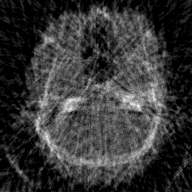
\includegraphics[width=\tempdima,height=\tempdima]{figures/experiments/recon_head/fdk40_slice_d.png}
                                                };
                                                \spy [yellow] on (0.45,-0.10) in node [left,yellow] at (1.2, 1.0);
                                        \end{scope}
                                \end{tikzpicture}
                        \end{subfigure}
                        \begin{subfigure}{0.22\linewidth}
                                \begin{tikzpicture}
                                        \begin{scope}[spy using outlines={rounded rectangle, magnification=2, width=1.0cm, height=0.75cm, connect spies}]
                                                \node[inner sep=0pt] {
                                                        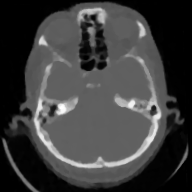
\includegraphics[width=\tempdima,height=\tempdima]{figures/experiments/recon_head/jrmtv40_slice_d.png}
                                                };
                                                \spy [yellow] on (0.45,-0.10) in node [left,yellow] at (1.2, 1.0);
                                        \end{scope}
                                \end{tikzpicture}
                        \end{subfigure}
                        \begin{subfigure}{0.22\linewidth}
                                \begin{tikzpicture}
                                        \begin{scope}[spy using outlines={rounded rectangle, magnification=2, width=1.0cm, height=0.75cm, connect spies}]
                                                \node[inner sep=0pt] {
                                                        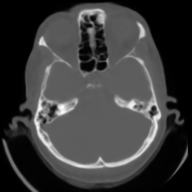
\includegraphics[width=\tempdima,height=\tempdima]{figures/experiments/recon_head/jrmadm40_slice_d.png}
                                                };
                                                \spy [yellow] on (0.45,-0.10) in node [left,yellow] at (1.2, 1.0);
                                        \end{scope}
                                \end{tikzpicture}
                        \end{subfigure}
                        \begin{subfigure}{0.22\linewidth}
                                \begin{tikzpicture}
                                        \begin{scope}[spy using outlines={rounded rectangle, magnification=2, width=1.0cm, height=0.75cm, connect spies}]
                                                \node[inner sep=0pt] {
                                                        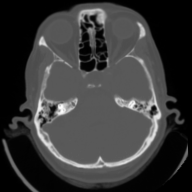
\includegraphics[width=\tempdima,height=\tempdima]{./figures/experiments/recon_head/gt_slice_d.png}
                                                };
                                                \spy [yellow] on (0.45,-0.10) in node [left,yellow] at (1.2, 1.0);
                                        \end{scope}
                                \end{tikzpicture}
                        \end{subfigure}
                \end{minipage}

                \noindent
                \begin{minipage}[c]{0.01\linewidth}
                        \centering
                        \rotatebox{90}{\footnotesize 20 views }
                \end{minipage}%
                \begin{minipage}[c]{0.99\linewidth}
                        \centering
                        \begin{subfigure}{0.22\linewidth}
                                \begin{tikzpicture}
                                        \begin{scope}[spy using outlines={rounded rectangle, magnification=2, width=1.0cm, height=0.75cm, connect spies}]
                                                \node[inner sep=0pt] {
                                                        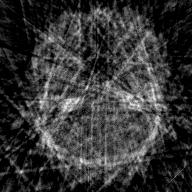
\includegraphics[width=\tempdima,height=\tempdima]{figures/experiments/recon_head/fdk20_slice_d.png}
                                                };
                                                \spy [yellow] on (0.45,-0.10) in node [left,yellow] at (1.2, 1.0);
                                        \end{scope}
                                \end{tikzpicture}
                                \caption{FDK}
                        \end{subfigure}
                        \begin{subfigure}{0.22\linewidth}
                                \begin{tikzpicture}
                                        \begin{scope}[spy using outlines={rounded rectangle, magnification=2, width=1.0cm, height=0.75cm, connect spies}]
                                                \node[inner sep=0pt] {
                                                        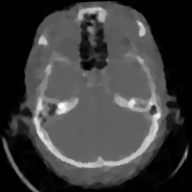
\includegraphics[width=\tempdima,height=\tempdima]{figures/experiments/recon_head/jrmtv20_slice_d.png}
                                                };
                                                \spy [yellow] on (0.45,-0.10) in node [left,yellow] at (1.2, 1.0);
                                        \end{scope}
                                \end{tikzpicture}
                                \caption{JRM-TV}
                        \end{subfigure}
                        \begin{subfigure}{0.22\linewidth}
                                \begin{tikzpicture}
                                        \begin{scope}[spy using outlines={rounded rectangle, magnification=2, width=1.0cm, height=0.75cm, connect spies}]
                                                \node[inner sep=0pt] {
                                                        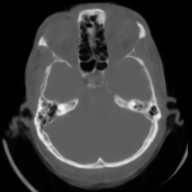
\includegraphics[width=\tempdima,height=\tempdima]{figures/experiments/recon_head/jrmadm20_slice_d.png}
                                                };
                                                \spy [yellow] on (0.45,-0.10) in node [left,yellow] at (1.2, 1.0);
                                        \end{scope}
                                \end{tikzpicture}
                                \caption{JRM-ADM}
                        \end{subfigure}
                        \begin{subfigure}{0.22\linewidth}
                                \begin{tikzpicture}
                                        \begin{scope}[spy using outlines={rounded rectangle, magnification=2, width=1.0cm, height=0.75cm, connect spies}]
                                                \node[inner sep=0pt] {
                                                        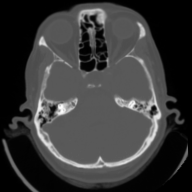
\includegraphics[width=\tempdima,height=\tempdima]{figures/experiments/recon_head/gt_slice_d.png}
                                                };
                                                \spy [yellow] on (0.45,-0.10) in node [left,yellow] at (1.2, 1.0);
                                        \end{scope}
                                \end{tikzpicture}
                                \caption{GT}
                        \end{subfigure}
                \end{minipage}

                \caption{GT and reconstructions (axial plane) for motion-affected sparse-view CBCT: results are shown for 40- and 20-view acquisition settings.}
        \end{figure}

\end{frame}